\documentclass{article}
\usepackage{amsmath}
\usepackage{graphicx}

\begin{document}

\title{An Expedition to The Valley of Genomics}
\author{Your Name}
\date{\today}

\maketitle



\section{29-05-2023}
\subsection{Commits}
\paragraph{Commit: bd81b50}
Commit Message: Hoy hicimos un workflow en el que cada commit se va guardado en el diario de laboratorio, con su id y con su mensaje. También se genera una sección de figuras para las figuras que fueron generadas en esa sesión

\paragraph{Commit: 7997396}
Commit Message: pruebo figura

\paragraph{Commit: 50ff4b4}
Commit Message: pruebo figura

\paragraph{Commit: 459b400}
Commit Message: ol

\paragraph{Commit: 1d47914}
Commit Message: prueba

\paragraph{Commit: ba9ba18}
Commit Message: prueba

\paragraph{Commit: 6029931}
Commit Message: prueba

\paragraph{Commit: 2b666e3}
Commit Message: prueba

\paragraph{Commit: b987caa}
Commit Message: prueba

\paragraph{Commit: 39adf1f}
Commit Message: prueba

\paragraph{Commit: 2c3ca23}
Commit Message: prueba

%CommitsEnd
\subsection{Figures}

\begin{figure}[h] \centering 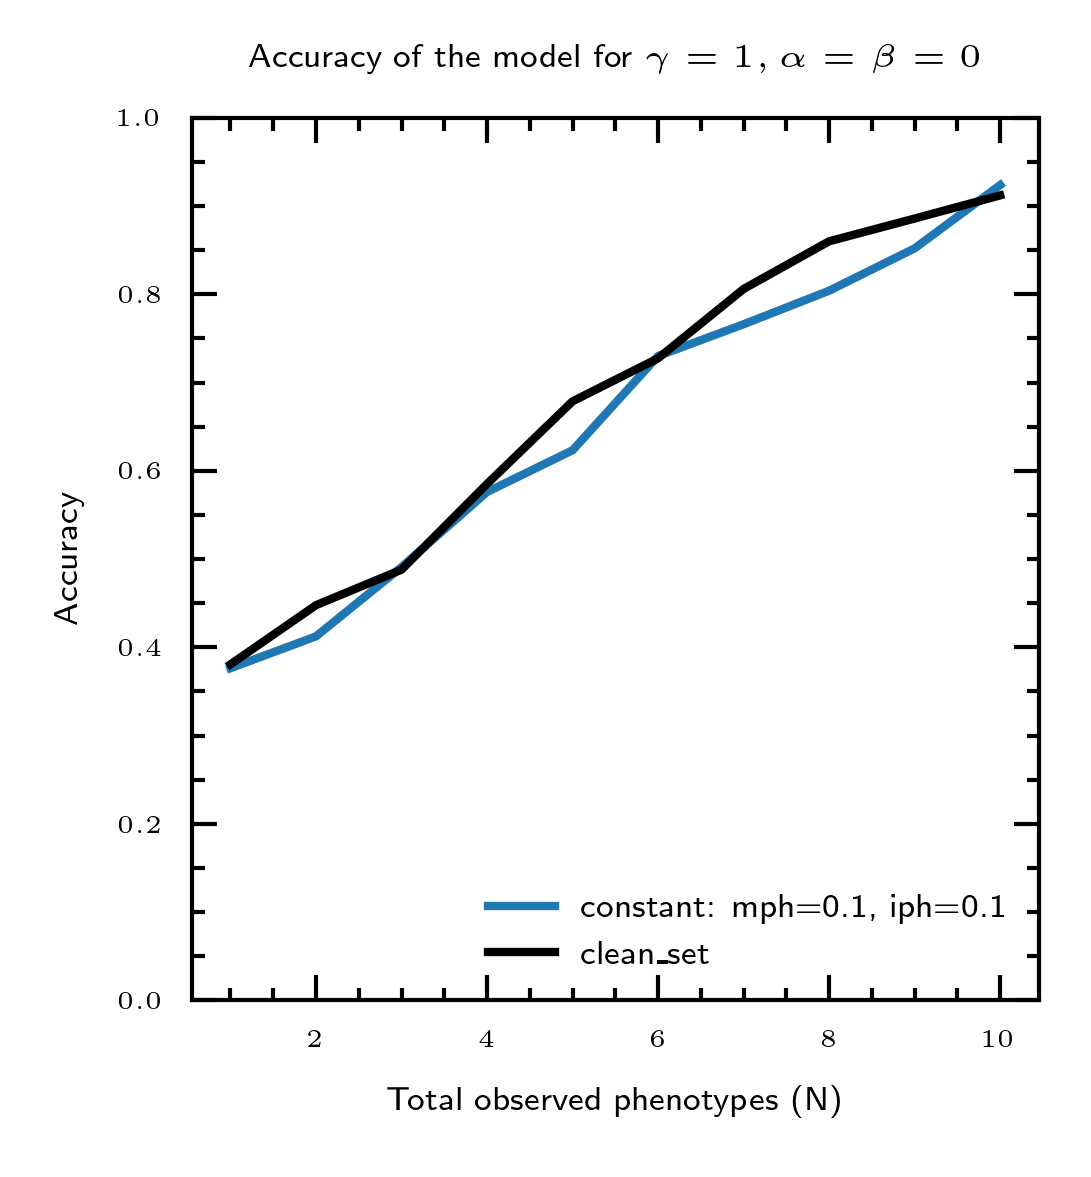
\includegraphics{jp.png} \caption{Caption for jp.png.} \end{figure}
\begin{figure}[h] \centering 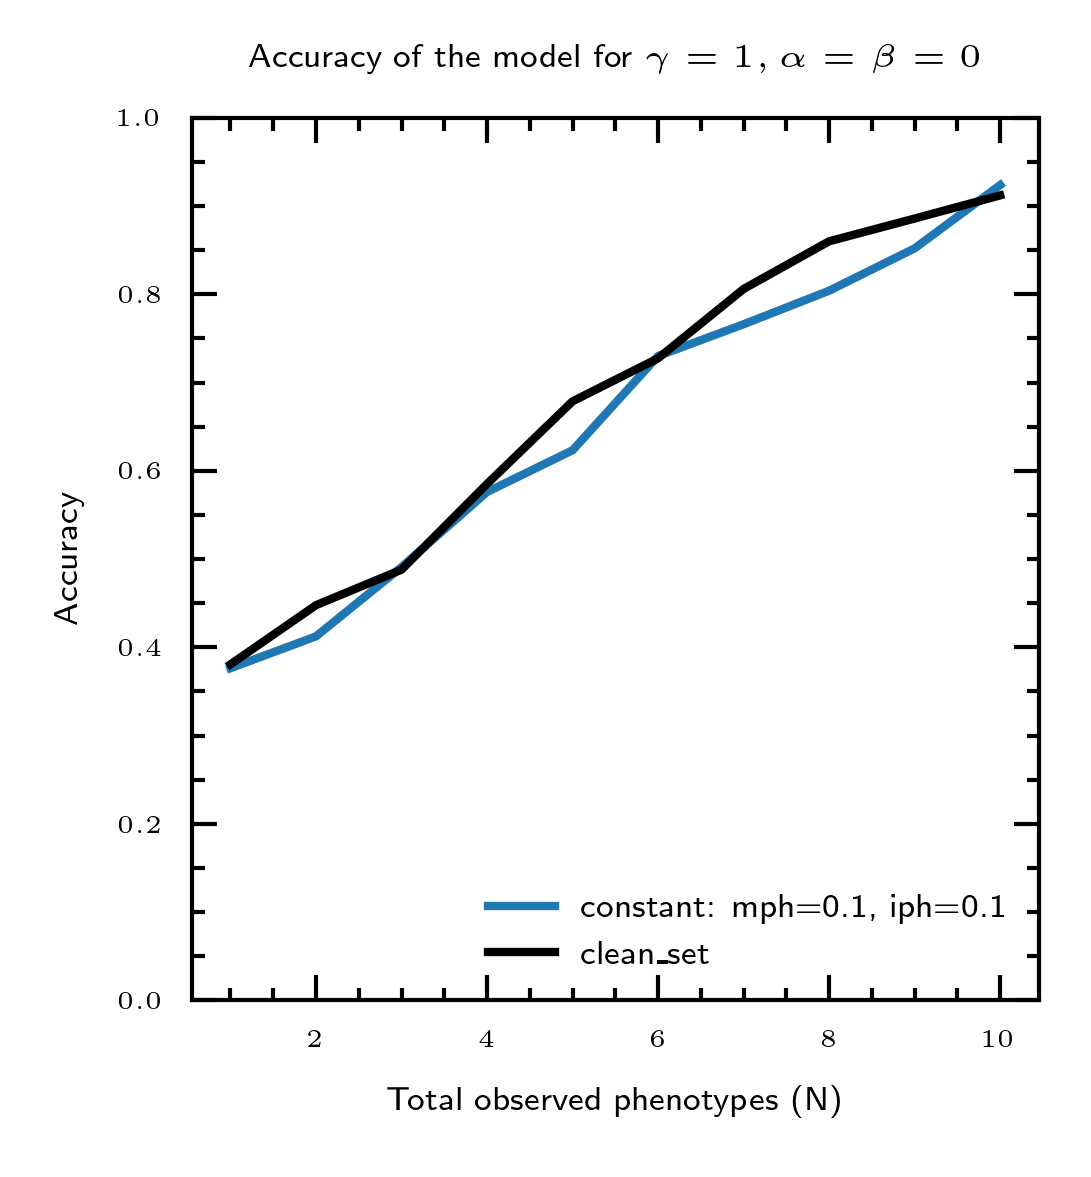
\includegraphics{pepe.png} \caption{Caption for pepe.png.} \end{figure}
%FiguresEnd
\subsection{Bibliography}
\subsection{Thoughts}

\end{document}

